\documentclass[12pt]{article}
\usepackage{enumitem}
\usepackage[letterpaper,left=2cm,right=2cm,top=2cm,bottom=2cm]{geometry}
\usepackage{tikz-cd,amsmath,amssymb}
\usepackage{graphicx}
\newenvironment{QandA}
{
	\begin{enumerate}[label=\normalfont\arabic*.,leftmargin=2em,rightmargin=2em]\normalfont
	}
	{
	\end{enumerate}
}
\newenvironment{codelalala}{}{}
\newenvironment{answered}{\setlength{\parindent}{1em}\par\normalfont}{}
\usepackage{lipsum}
\pagestyle{empty}
\title{CSE 573 Fall 2018 Project 2}
\author{Pratik Pravin Kubal}
\date{UB Person Number: 50290804}
\pagestyle{plain}
\begin{document}
	\noindent%
	\maketitle
	\begin{QandA}
		\item Image Features and Homography
		{
		\begin{enumerate}
		\item {
			Given two images mountain1.jpg and mountain2.jpg
, extract SIFT features and draw the keypoints for both images. Include the resulting two images (task1$\_$sift1.jpg, task1$\_$sift2.jpg) in the report.\\
		\begin{answered}
		SIFT Features are patiented in OpenCV and this task took most of my time since I had to build OpenCV from source with custom flags. I have used Rich Keypoints to display the detected keypoints. Refer to Figure \ref{sift-detection} for the output.
		\begin{verbatim}
		img1_g = cv2.cvtColor(img1.copy(),cv2.COLOR_BGR2GRAY)
		img2_g = cv2.cvtColor(img2.copy(),cv2.COLOR_BGR2GRAY)
		
		sift = cv2.xfeatures2d.SIFT_create()
keypoints_img1 = sift.detect(img1.copy(),None)
keypoints_img2 = sift.detect(img2.copy(),None)

display_img1=cv2.drawKeypoints(img1_g.copy(),keypoints_img1.copy(),
img1.copy(),flags=cv2.DRAW_MATCHES_FLAGS_DRAW_RICH_KEYPOINTS)
display_img2=cv2.drawKeypoints(img2_g.copy(),keypoints_img2.copy(),
img2.copy(),flags=cv2.DRAW_MATCHES_FLAGS_DRAW_RICH_KEYPOINTS)
		\end{verbatim}
	\begin{figure}
		\centering
  			\fbox{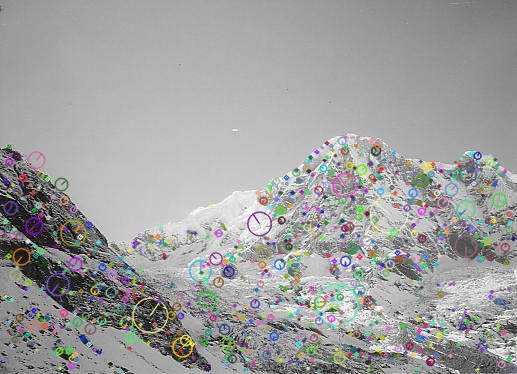
\includegraphics[scale=0.50]{./task1_sift1.jpg}
  					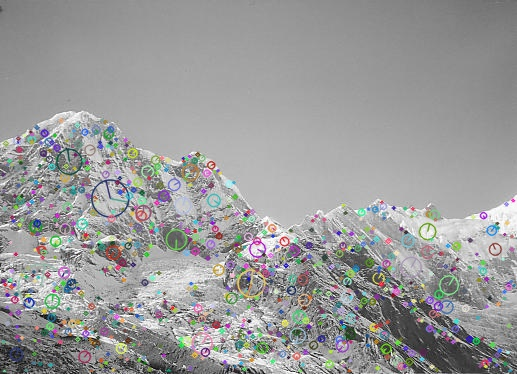
\includegraphics[scale=0.50]{./task1_sift2.jpg}}
  			\caption{SIFT Feature Detection - Keypoints}
  		\label{sift-detection}
	\end{figure}
		\end{answered}		
		}
		\item {
 Match the keypoints using k-nearest neighbour (k=2), i.e., for a keypoint in the left image, finding the  best 2  matches  in  the right image. Filter  good  matches  satisfy m.distance <0.75 n.distance ,  where m is the first match and n is the second match. Draw the match image using cv2.drawMatches for all matches (your match image should contain both inliers and outliers). Include the result image( task1$\_$matches$\_$knn.jpg) in the report. 	\\
	\begin{answered}
				The output of this task can be seen in Figure \ref{sift-knn}. I have used Flann based matcher instead of a Brute force approach.
				\begin{verbatim}
				keypoints_img1knn, desc1 = sift.detectAndCompute(img1_g.copy(),None)
keypoints_img2knn, desc2 = sift.detectAndCompute(img2_g.copy(),None)

FLANN_INDEX_KDTREE = 1
index_params = dict(algorithm = FLANN_INDEX_KDTREE, trees = 50)
search_params = dict(checks=50000)

flann = cv2.FlannBasedMatcher(index_params,search_params)

matches = flann.knnMatch(desc1,desc2,k=2)
ratioTestM=[]

for i,(m,n) in enumerate(matches):
    if m.distance < 0.75*n.distance:
        ratioTestM.append([m])
        
img3 = cv2.drawMatchesKnn(img1_g.copy(),keypoints_img1knn.copy(),img2_g.copy(),
keypoints_img2knn.copy(),ratioTestM,None,flags =2)
				\end{verbatim}
	\begin{figure}
		\centering
  			\fbox{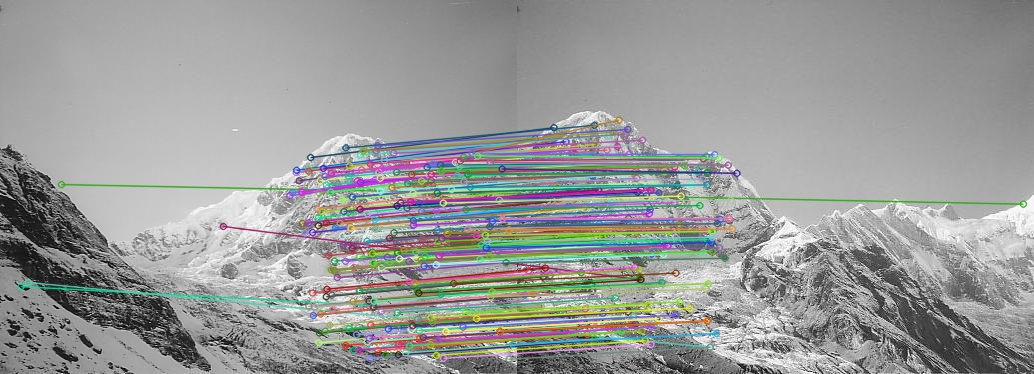
\includegraphics[scale=0.50]{./task1_matches_knn.jpg}}
  			\caption{SIFT Feature Detection - KNN}
  		\label{sift-knn}
	\end{figure}
		\end{answered}	
		}
		
		\item {
Compute the homography matrix H (with  RANSAC) from the first image to the second image. Include the matrix values in the report.
\begin{answered}
		The Homography Matrix found is as follows.
		\[
		H = 
		\begin{bmatrix}
		1.59917  & -0.2983217  & -378.50952 \\
    	0.430010  & 1.38050  & -179.18731 \\
    	0.001155 & -0.0001214  & 1
		\end{bmatrix}
		\]
		\begin{verbatim}
ratioTestM = np.array(ratioTestM)
src_pts = np.float32([keypoints_img1knn[m.queryIdx].pt for m in ratioTestM.flatten()])
dst_pts = np.float32([keypoints_img2knn[m.trainIdx].pt for m in ratioTestM.flatten()])
# ,maxIters=50
H, mask = cv2.findHomography(src_pts,dst_pts, cv2.RANSAC,1,maxIters=2000000000)
matchesMask = mask.ravel().tolist()
		\end{verbatim}
		\end{answered}
		}
		\item {
Draw the match image for around 10 random matches using only inliers. Include the result image (task1$\_$matches.jpg) in the report.
		\begin{answered}
		The code which I used was as follows and the output image can be seen in Figure \ref{sift-final-matches}
		\begin{verbatim}
		rand10matchesMask = []
inlier_idx = []
for i in range(0,len(matchesMask)):
    if(matchesMask[i] == 1):
        inlier_idx.append(i)
rand10Places = np.random.choice(inlier_idx,10,replace=False)
for i in range(0,len(matchesMask)):
    if((i == rand10Places).any()):
        rand10matchesMask.append(1)
    else:
        rand10matchesMask.append(0)

draw_params = dict(matchColor = (0,255,0),
                   singlePointColor = None,
                   matchesMask = rand10matchesMask,
                   flags = 2)

img4 = cv2.drawMatches(img1_g.copy(),keypoints_img1knn,img2_g.copy(),keypoints_img2knn,ratioTestM.flatten(),None,**draw_params)
		\end{verbatim}
			\begin{figure}
		\centering
  			\fbox{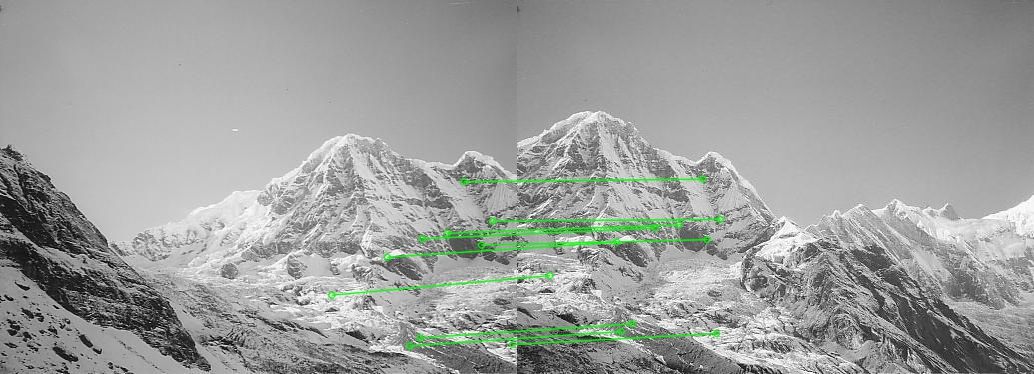
\includegraphics[scale=0.50]{./task1_matches.jpg}}
  			\caption{task1$\_$matches.jpg}
  		\label{sift-final-matches}
	\end{figure}
		\end{answered}
		}
		\item {
Warp the first image to the second image using H
. The resulting image should contain all pixels in mountain1.jpg and mountain2.jpg. Include the result image (task1$\_$pano.jpg) in the report. 		
		\begin{answered}
		I have researched multiple sites as to work on this problem. The figure of the output can be seen in Fig.  \ref{sift-pano}
		\begin{verbatim}
		h,w = np.shape(img1_g)
corners = np.array([
  [0,0],
  [0,h-1],
  [w-1,h-1],
  [w-1,0]
])
corners = cv2.perspectiveTransform(np.float32([corners]),H)[0]
bx, by, bwidth, bheight = cv2.boundingRect(corners)
translation = np.array([
  [1,0,-bx],
  [0,1,-by],
  [0,0,1]
])
H2 = np.dot(translation,H)
warpImg = cv2.warpPerspective(img1_g.copy(),H2,((w*2),bheight+15))
warpImg[bheight-h+15:bheight-h+15+h,w:]=img2_g.copy()
		\end{verbatim}
		Since the offset of the Homography matrix is negative, and not 0,0 we bring the corners which are outside inside by using perspective projection.
					\begin{figure}
		\centering
  			\fbox{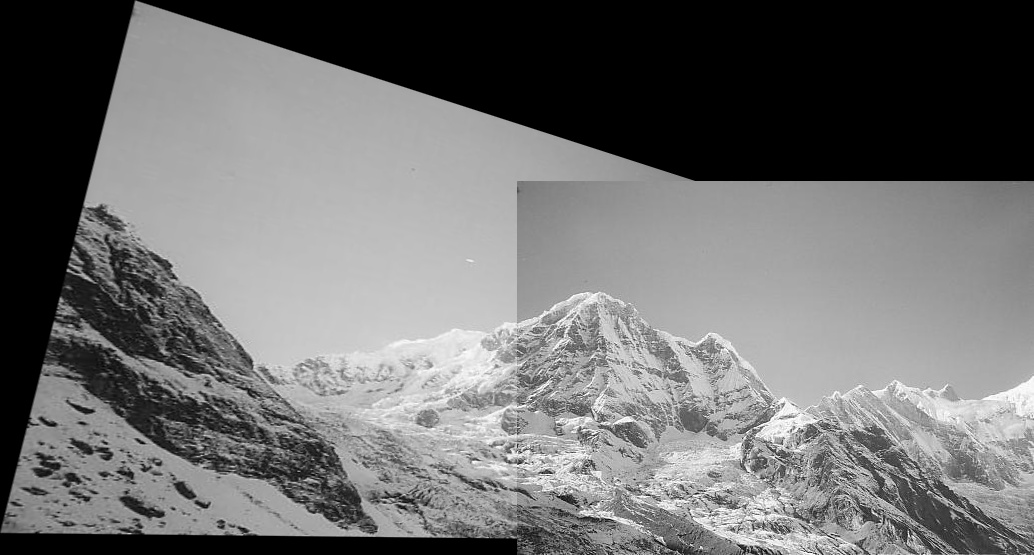
\includegraphics[scale=0.30]{./task1_pano.jpg}}
  			\caption{task1$\_$pano.jpg}
  		\label{sift-pano}
	\end{figure}
		\end{answered}
		}
		\end{enumerate}
		}
	\item {
	Epipolar Geometry
	\begin{enumerate}
	\item {
	Given two images tsucuba$\_$left.png and tsucuba$\_$right.png, do the same process for Task1.1 and 1.2. Include the three images (2 for task 1.1 and 1 for task 1.2) (task2$\_$sift1.jpg,task2$\_$sift2.jpg, task2$\_$matches$\_$knn.jpg) in the report.
	\begin{answered}
	The figures can be found in Figure \ref{task21},\ref{task22},\ref{task23}. Concise code is as follows,\\
	\begin{verbatim}
	sift = cv2.xfeatures2d.SIFT_create()
keypoints_img_left = sift.detect(img_left_g.copy(),None)
keypoints_img_right = sift.detect(img_right_g.copy(),None)
	\end{verbatim}
	\begin{verbatim}
	
keypoints_img_leftknn, desc1 = sift.detectAndCompute(img_left_g.copy(),None)
keypoints_img_rightknn, desc2 = sift.detectAndCompute(img_right_g.copy(),None)

FLANN_INDEX_KDTREE = 1
index_params = dict(algorithm = FLANN_INDEX_KDTREE, trees = 50)
search_params = dict(checks=50000)

flann = cv2.FlannBasedMatcher(index_params,search_params)

matches = flann.knnMatch(desc1,desc2,k=2)
ratioTestM=[]

for i,(m,n) in enumerate(matches):
    if m.distance < 0.75*n.distance:
        ratioTestM.append([m])
	\end{verbatim}
	\begin{figure}
		\centering
  			\fbox{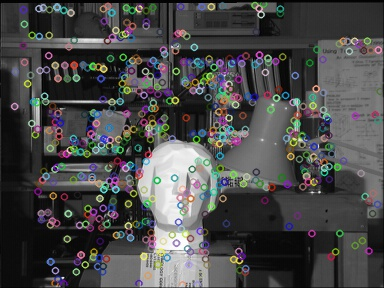
\includegraphics[scale=0.50]{./task2_sift1.jpg}}
  			\caption{task2$\_$sift1.jpg}
  		\label{task21}
	\end{figure}
		\begin{figure}
		\centering
  			\fbox{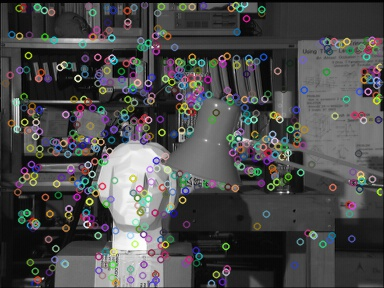
\includegraphics[scale=0.50]{./task2_sift2.jpg}}
  			\caption{task2$\_$sift2.jpg}
  		\label{task22}
	\end{figure}
			\begin{figure}
		\centering
  			\fbox{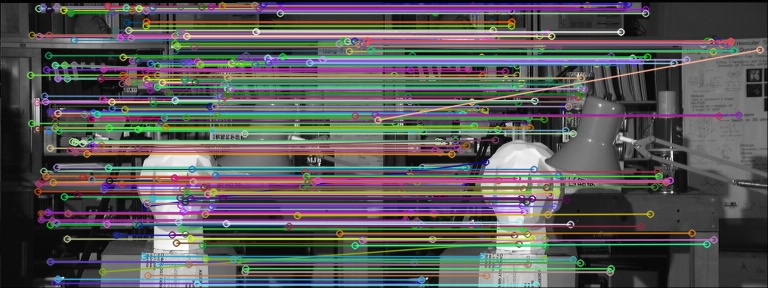
\includegraphics[scale=0.50]{./task2_matches_knn.jpg}}
  			\caption{task2$\_$matches$\_$knn.jpg}
  		\label{task23}
	\end{figure}
	\end{answered}
	}
	\item {
Computer the fundamental matrix F (with RANSAC). Include the matrix values in the report.
	\begin{answered}
		The Fundamental Matrix found is as follows.
		\[
		F = 
		\begin{bmatrix}
		5.62983212\times10^{-06}  & -7.11772433\times10^{-04}  & 9.46307599\times10^{-02} \\
    	6.55527783\times10^{-04}  & -7.07029260\times10^{-05}  & -7.70491291\times10^{-02} \\
    	-9.14620736\times10^{-02} & 8.26304703\times10^{-02}  & 1
		\end{bmatrix}
		\]
	\end{answered}	
	}
	\item {
Randomly  select  10 inlier match  pairs.   For  each  keypoint  in  the  left  image,  compute  the epiline  and  draw  on  the  right  image.   For  each  keypoint  in  the  right  image,  compute  the epiline and draw on the left image [Using different colors for different match pairs, but the same color for epilines on the left and right images with the same match pair.]  Include two images (task2$\_$epi$\_$right.jpg,task2$\_$epi$\_$left.jpg) with epilines in the report. 	
\begin{answered}
I used an openCV function to draw the lines. The code is as follows: The Figures can be found in Figure \ref{epi-left} and \ref{epi-right}
\begin{verbatim}
rand10matchesMask = []
inlier_idx = []
for i in range(0,len(matchesMask)):
    if(matchesMask[i] == 1):
        inlier_idx.append(i)
rand10Places = np.random.choice(inlier_idx,10+1,replace=False)
for i in range(0,len(matchesMask)):
    if((i == rand10Places).any()):
        rand10matchesMask.append(1)
    else:
        rand10matchesMask.append(0)
\end{verbatim}
\begin{verbatim}

rand10matchesMask= np.array(rand10matchesMask)

left_pts = left_pts[rand10matchesMask==1]
right_pts = right_pts[rand10matchesMask == 1]

linesonLeft = cv2.computeCorrespondEpilines(right_pts.reshape(-1,1,2), 2,F)
linesonLeft = linesonLeft.reshape(-1,3)
img5,img6 = drawlines(img_left_g,img_right_g,linesonLeft,left_pts,right_pts)

linesonRight = cv2.computeCorrespondEpilines(left_pts.reshape(-1,1,2), 1,F)
linesonRight = linesonRight.reshape(-1,3)
img3,img4 = drawlines(img_right_g,img_left_g,linesonRight,right_pts,left_pts)
\end{verbatim}
\begin{verbatim}
def drawlines(img1,img2,lines,pts1,pts2):
    # Reference CV2 Documentation
    # https://docs.opencv.org/3.1.0/da/de9/tutorial_py_epipolar_geometry.html
    import cv2
    import numpy as np
    r,c = img1.shape
    img1 = cv2.cvtColor(img1,cv2.COLOR_GRAY2BGR)
    img2 = cv2.cvtColor(img2,cv2.COLOR_GRAY2BGR)
    colDict = {1:(74, 208, 197),
               2:(140, 20, 143),
               3:(179, 241, 184),
               4:(23, 82, 85),
               5:(135, 0, 55),
               6:(255, 255, 255),
               7:(157, 127, 31),
               8:(198, 167, 158),
               9:(124, 237, 58),
               10:(100, 194, 116)}
    i=1
    for r,pt1,pt2 in zip(lines,pts1,pts2):
        color = colDict.get(i)
        x0,y0 = map(int, [0, -r[2]/r[1] ])
        x1,y1 = map(int, [c, -(r[2]+r[0]*c)/r[1] ])
        img1 = cv2.line(img1, (x0,y0), (x1,y1), color,1)
        img1 = cv2.circle(img1,tuple(pt1),5,color,-1)
        img2 = cv2.circle(img2,tuple(pt2),5,color,-1)
        i+=1
    return img1,img2
\end{verbatim}
			\begin{figure}
		\centering
  			\fbox{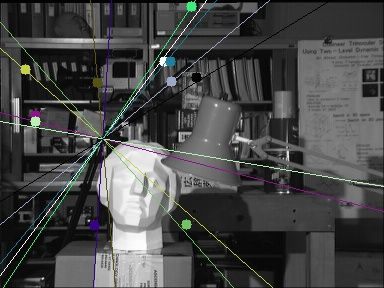
\includegraphics[scale=0.50]{./task2_epi_left.jpg}}
  			\caption{task2$\_$epi$\_$left.jpg}
  		\label{epi-left}
	\end{figure}
				\begin{figure}
		\centering
  			\fbox{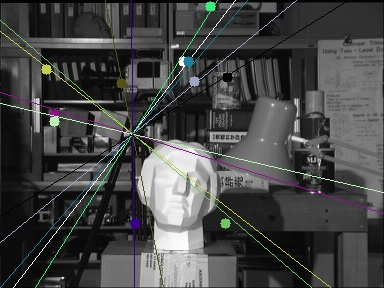
\includegraphics[scale=0.50]{./task2_epi_right.jpg}}
  			\caption{task2$\_$epi$\_$right.jpg}
  		\label{epi-right}
	\end{figure}
\end{answered}
	}
	\item {
Compute  the  disparity  map  for tsucuba$\_$left.png and tsucuba$\_$right.png. Include the disparity image (task2$\_$disparity.jpg) in the report. 
	\begin{answered}
	The Figures can be found in fig \ref{disparity} and the code is as follows:
	\begin{verbatim}
	stereo = cv2.StereoBM_create(numDisparities=64, blockSize=27)
disparity = stereo.compute(img_left_g,img_right_g)
disparity_norm = normImage(disparity)
disparity_norm = np.asanyarray(np.dot(disparity_norm,255),dtype='int32')
cv2.imwrite('2/task2_disparity.jpg',disparity_norm)
	\end{verbatim}
					\begin{figure}
		\centering
  			\fbox{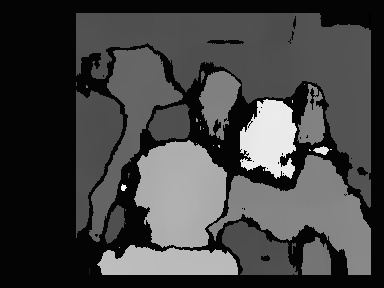
\includegraphics[scale=0.50]{./task2_disparity.jpg}}
  			\caption{task2$\_$disparity.jpg}
  		\label{disparity}
	\end{figure}
	
	\end{answered}	
	}
	\end{enumerate}
		}
	\item {
	K-means Clustering
	\begin{enumerate}
	 \item {Classify N= 10 samples according to nearest $\mu_i$(i= 1,2,3). Plot the results by coloring the empty triangles in red, blue or green. Include the classification vector and the classification plot (task3$\_$iter1a.jpg) in the report.
	 \begin{answered}
	 The Classification vector is as follows:\\
	 $\{0: 0, 1: 0, 2: 2, 3: 0, 4: 1, 5: 0, 6: 0, 7: 2, 8: 0, 9: 0\}$\\
	 The output of the first iteration can be seen in Fig \ref{img31a}:
	 					\begin{figure}
		\centering
  			\fbox{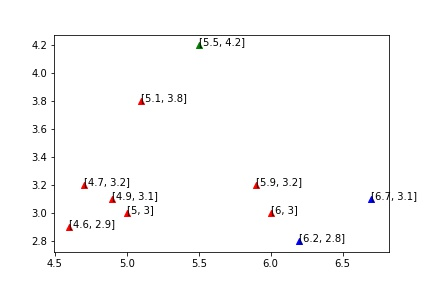
\includegraphics[scale=0.60]{./task3_iter1_a.jpg}}
  			\caption{task3$\_$iter1$\_$a.jpg}
  		\label{img31a}
	\end{figure}
	 \end{answered} }
	 \item {
Recompute $\mu_i$. Plot the updated $\mu_i$ in solid circle in red, blue, and green respectively. Include the updated $\mu_i$ values and the plot in the report(task3$\_$iter1$\_$b.jpg)
\begin{answered}
The updated values are:
		\[
		\mu_i = 
		\begin{bmatrix}
		5.1714 & 3.1714 \\
		5.5 & 4.2 \\
		6.45 & 2.95
		\end{bmatrix}
		\]
		And the figure is at \ref{img32}

	 					\begin{figure}
		\centering
  			\fbox{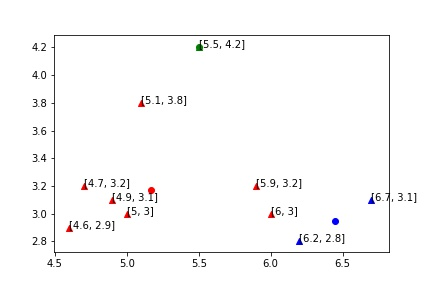
\includegraphics[scale=0.60]{./task3_iter1_b.jpg}}
  			\caption{task3$\_$iter1$\_$b.jpg}
  		\label{img32}
	\end{figure}
	The Functions constructed are as follows:
	\begin{verbatim}
	def eucl_distance(point,centroid):
    import numpy as np
    return np.sqrt(np.sum(np.square(centroid - point)))
	\end{verbatim}
	\begin{verbatim}
	
def kmeans(points,centroids,point_centroid_dict):
    import numpy as np
    points = np.matrix(points)
    centroids = np.matrix(centroids)
    i = 0
    for point in points:
        minArray = []
        for centroid in centroids:
            minArray.append(eucl_distance(point,centroid))
        point_centroid_dict.update({i:minArray.index(np.min(minArray))})
        i +=1
    return point_centroid_dict
	\end{verbatim}
	\begin{verbatim}
	def updateCentroids(points,centroids,point_centroid_dict):
    import numpy as np
    cluster_centroid_dict={}
    for i,point in enumerate(points):
        cluster = point_centroid_dict.get(i)
        clusterCentroidData=cluster_centroid_dict.get(cluster)
        if(clusterCentroidData is None):
            running_x = point[0]
            running_y = point[1]
            cluster_centroid_dict.update({point_centroid_dict.get(i):
            [[running_x],[running_y]]})
        else:
           prev_running_x,prev_running_y = clusterCentroidData.copy()
           prev_running_x.append(point[0])
           prev_running_y.append(point[1])
           cluster_centroid_dict.update({point_centroid_dict.get(i):
           s[prev_running_x,prev_running_y]})
    # Recomputing Clusters
    newCentroids = centroids
    for i,_ in enumerate(centroids):
        xcords,ycords = cluster_centroid_dict.get(i)
        newCentroids[i][0] = np.mean(xcords)
        newCentroids[i][1] = np.mean(ycords)
    return newCentroids
	\end{verbatim}
\end{answered}	 
	 }
	\item {
For a second iteration, plot the classification plot and updated μ$_i$ plot for the second iteration. Include the classification vector and updated $\mu_i$ values and these two plots (task3$\_$iter2$\_$a.jpg,task3$\_$iter2$\_$b.jpg) in the report.
\begin{answered}
The classification vector is as follows:\\
$\{0: 2, 1: 0, 2: 2, 3: 0, 4: 1, 5: 0, 6: 0, 7: 2, 8: 1, 9: 2\}$\\
	 \begin{figure}
		\centering
  			\fbox{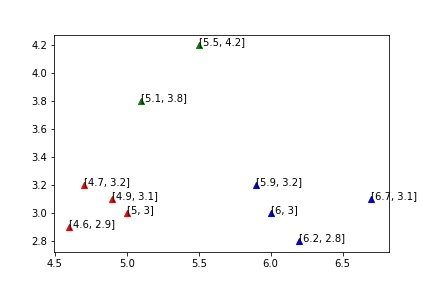
\includegraphics[scale=0.60]{./task3_iter2_a.jpg}}
  			\caption{task3$\_$iter2$\_$a.jpg}
  		\label{img32}
	\end{figure}		
		 \begin{figure}
		\centering
  			\fbox{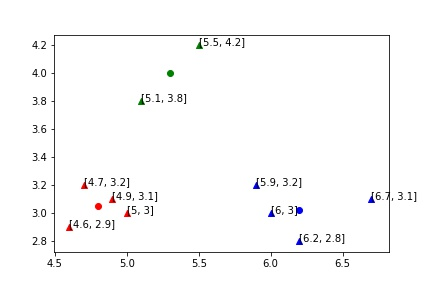
\includegraphics[scale=0.60]{./task3_iter2_b.jpg}}
  			\caption{task3$\_$iter2$\_$b.jpg}
  		\label{img32}
	\end{figure}
\end{answered}	
	}	
	The updated $\mu_i$ values are as follows: 
	 \[
		\mu_i = 
		\begin{bmatrix}
		4.800 & 3.05 \\
		5.3 & 4.0 \\
		6.2 & 3.025
		\end{bmatrix}
		\]
	 \item {
Color Quantization
\begin{answered}
The functions which I used are as follows:
\begin{verbatim}
def eucl_distance3d(point,centroid):
    # point = [r[0][0],g[0][0],b[0][0]]
    import numpy as np
    return np.sqrt(np.sum(np.square(centroid - point)))
\end{verbatim}
\begin{verbatim}
def kmeans3d(raster,centroids,point_centroid_dict):
    import numpy as np
    raster = np.array(raster)
    centroids = np.matrix(centroids)
    for h in range(0,np.shape(raster)[0]):
        rowDict={}
        for w in range(0,np.shape(raster)[1]):
            minArray = []
            for centroid in centroids:
                minArray.append(eucl_distance3d(raster[h][w],centroid))
            rowDict.update({w:minArray.index(np.min(minArray))})
        point_centroid_dict.update({h:rowDict})
    return point_centroid_dict
\end{verbatim}
\begin{verbatim}
def updateCentroids3d(raster,centroids,point_centroid_dict):
    import numpy as np
    cluster_centroid_dict={}
    for h in range(0,np.shape(raster)[0]):
        for w in range(0,np.shape(raster)[1]):
            cluster = point_centroid_dict.get(h).get(w)
            clusterCentroidData=cluster_centroid_dict.get(cluster)
            if(clusterCentroidData is None):
                running_r = raster[h][w][0]
                running_g = raster[h][w][1]
                running_b = raster[h][w][2]
                cluster_centroid_dict.update({point_centroid_dict.get(h).
                get(w):[[running_r],[running_g],[running_b]]})
            else:
                prev_running_r,prev_running_g,prev_running_b = 
                clusterCentroidData.copy()
                prev_running_r.append(raster[h][w][0])
                prev_running_g.append(raster[h][w][1])
                prev_running_b.append(raster[h][w][2])
                cluster_centroid_dict.update({point_centroid_dict.
                get(h).get(w):[prev_running_r,prev_running_g,prev_running_b]})
    newCentroids = np.array(centroids)
    for i,_ in enumerate(centroids):
        if(cluster_centroid_dict.get(i) is not None):
            xcords,ycords,zcords = cluster_centroid_dict.get(i)
            newCentroids[i][0] = np.mean(xcords)
            newCentroids[i][1] = np.mean(ycords)
            newCentroids[i][2] = np.mean(zcords)
    return np.matrix(newCentroids)
\end{verbatim}
\begin{verbatim}
def quantaRaster(raster,point_centroid_dict,centroids):
    import numpy as np
    resultImage = []
    for h in range(0,np.shape(raster)[0]):
        holdRow =[]
        for w in range(0,np.shape(raster)[1]):
            r,g,b = np.array(centroids[point_centroid_dict.get(h).
            get(w)]).flatten()
            holdRow.append([r,g,b])
        resultImage.append(holdRow)
    return resultImage
\end{verbatim}
The Color Quantization images for k=3,5,10,20 are as follows in Figures \ref{baboon3}, \ref{baboon5}, \ref{baboon10},\ref{baboon20}.
		 \begin{figure}
		\centering
  			\fbox{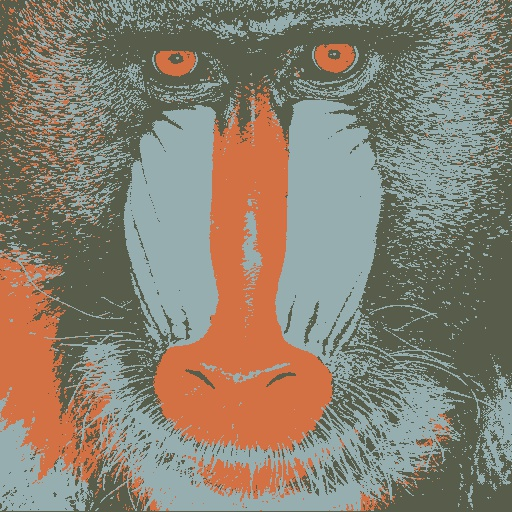
\includegraphics[scale=0.40]{./task3_baboon_3.jpg}}
  			\caption{task3$\_$baboon$\_$3.jpg}
  		\label{baboon3}
	\end{figure}
			 \begin{figure}
		\centering
  			\fbox{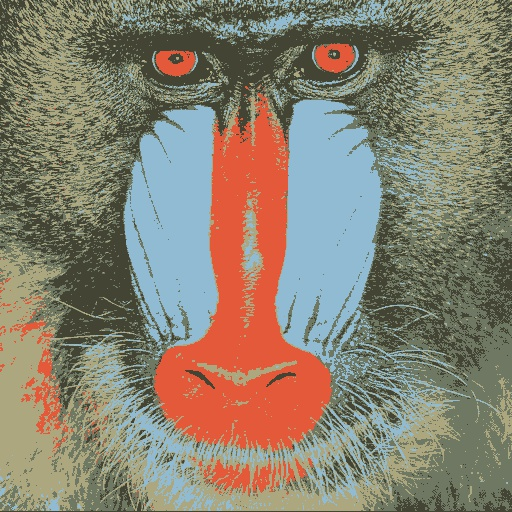
\includegraphics[scale=0.40]{./task3_baboon_5.jpg}}
  			\caption{task3$\_$baboon$\_$5.jpg}
  		\label{baboon5}
	\end{figure}
				 \begin{figure}
		\centering
  			\fbox{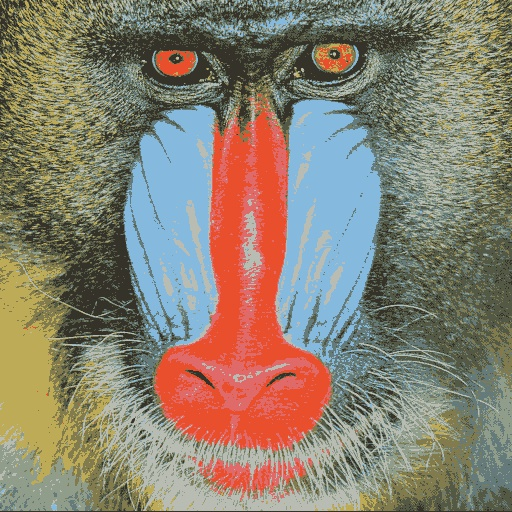
\includegraphics[scale=0.40]{./task3_baboon_10.jpg}}
  			\caption{task3$\_$baboon$\_$10.jpg}
  		\label{baboon10}
	\end{figure}
					 \begin{figure}
		\centering
  			\fbox{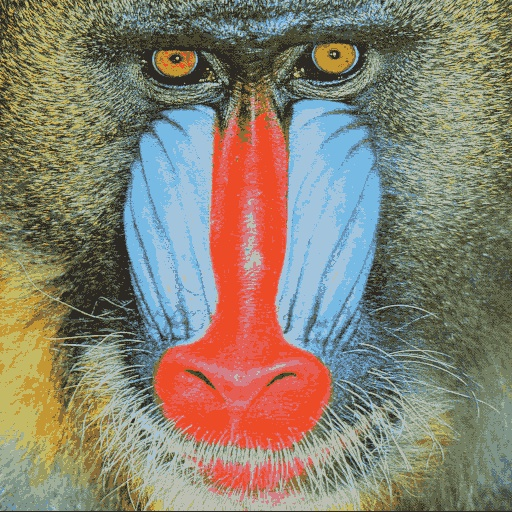
\includegraphics[scale=0.40]{./task3_baboon_20.jpg}}
  			\caption{task3$\_$baboon$\_$20.jpg}
  		\label{baboon20}
	\end{figure}
	\item {
	Gaussian Mixture Model
	\begin{answered}
	I used a EM based method to implement the GMM. I couldn't complete the whole method but I was about to complete the first task. After the first iteration I am getting the new $\mu_i$ as:
		 \[
		\mu_i = 
		\begin{bmatrix}
		5.3165079 & 3.21527292 \\
		5.61129795  & 3.38505 \\
		5.60443565 & 3.14420061
		\end{bmatrix}
		\]
		Here each row corresponds to one cluster.
	\end{answered}	
	}
\end{answered}	 
	 }
	\end{enumerate}
	}
\end{QandA}
\end{document}
